\clearpage

\section{Entropy Estimator}

\begin{tcolorbox}	
	\begin{tabular}{p{2.75cm} p{0.2cm} p{10.5cm}} 	
		\textbf{Header File}   &:& \texttt{"entropy\_estimator\_20180715.h"} \\
		\textbf{Source File}   &:& \texttt{"entropy\_estimator\_20180715.cpp"} \\
		\textbf{Version}       &:& 20180715 (Gustavo Anjos) \\
	\end{tabular}
\end{tcolorbox}


\subsection*{Input Parameters}

\begin{table}[h]
	\centering
	\begin{tabular}{|c|c|c|c|c|}
		\cline{1-4}
		\textbf{Parameter} & \textbf{Type} &\textbf{Values} &   \textbf{Default}& \\ \cline{1-4}
		nBits 	& int 	& $\geq$ 1 & Input Buffer Size \\ \cline{1-4}
		minWindow	 & int 	& ]0,nBits]  & Input Buffer Size \\ \cline{1-4} \cline{1-4}
	\end{tabular}
	\caption{Entropy estimator input parameters}
	\label{table:estimator_in_par}
\end{table}

\subsection*{Functional Description}
This block computes the entropy of a binary signal defined at the input, generating 
a file \texttt{"entropy\_est.txt"} with the mean and variance of the individual estimations.
The binary signal at the input is writen at the output of the estimator without changes.

\begin{figure}[h]
\subsection*{}
    \centerline{
       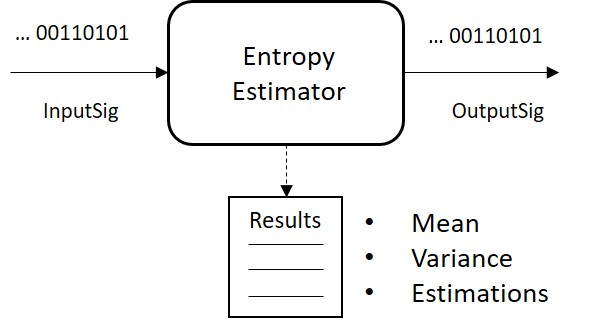
\includegraphics[scale=0.75]{figures/block_entropy_est.jpg}
    }
\end{figure}

\textbf{Mathematical Definition}: Defining \textit{p} as the probability of the 
outcome '1', the binary entropy \textit{h} is computed using the following expression

\begin{equation}
h = -p\log_2(p) - (1-p)\log_2(1-p)
\end{equation}  
   
\paragraph{}
\textbf{Parameters Description}: The parameter 'minWindow' allows the user to set the 
minimum window size for each individual estimation. If 'minWindow' is lower than the 
input buffer size, the estimator adjusts the window to the size of the input buffer, 
otherwise the window is rounded to a multiple of the input buffer size, ensuring always 
that the window is greater or equal than 'minWindow'. The total number of bits processed 
by the estimator is equal to the largest value that is a multiple of the window size and 
is not greater than the input parameter 'nBits'.

\subsection*{Input Signals}
\subparagraph*{Number:} 1
\subparagraph*{Type:} Binary

\subsection*{Output Signals}
\subparagraph*{Number:} 1
\subparagraph*{Type:} Binary

\subsection*{Methods}
\subparagraph*{}
entropy\_estimator(vector$<$Signal *$>$ \&InputSig, vector$<$Signal *$>$ \&OutputSig);
\subparagraph*{}
bool runBlock(void)
\subparagraph*{}
void setNumbBits(int n)
\subparagraph*{}
int getNumbBits(void)
\subparagraph*{}
void setMinWindowSize(int w)
\subparagraph*{}
int getMinWindowSize(void)






